
Today lecture is about linear dynamics control models. The main
difference is that on the one hand we will have a continuous state
and action space, and on the other hand we will assume a very
specific dynamics (linear) and costs (quadratic).

For a motivating example consider a helicopter with a simple
physical dynamics. The current height of the helicopter is a
function of the previous height and acceleration (we assume that we
discretize time).

Specifically, let $h_t$ be the height of the helicopter at time $t$,
$v_t$ its velocity, and $a_t$ the acceleration. (We will view the
problem as a one dimensional one.) The dynamics are set as follows,
\begin{align*}
h_{t+1} =& h_t +\tau v_t +\frac{1}{2} \tau^2(a_t-g)\\
v_{t+1} = & v_t +\tau (a_t-g)
\end{align*}
where $\tau$ is the time step and $g$ is the gravity.

We can write it as a linear dynamics as follows
\[
\underbrace{
\begin{bmatrix}
h_{t+1}\\
v_{t+1}
\end{bmatrix}}_{x_{t+1}}
= \underbrace{
\begin{bmatrix}
1&\tau\\
0&1
\end{bmatrix}
}_A
\underbrace{
\begin{bmatrix}
h_{t}\\
v_{t}
\end{bmatrix}
}_{x_t} +
\underbrace{\begin{bmatrix}
\frac{1}{2}\tau^2\\
\tau
\end{bmatrix}
}_B
(a_t-g)
\]
This gives the Linear Time Invariant (LTI) system:
\[
x_{t+1}=Ax_t+Bu_t
\]

We described the dynamics of the system. This gives us a way to
start at an initial state $x_0$ and reach a final state $x_T$. In
addition to reaching the final state $x_T$ we would like to minimize
some cost function, which depends on the states and actions. We will
look at {\em quadratic cost} function $J(\cdot)$. Given an initial
state $x_0$ and a sequence of actions $u=(u_1, \ldots , u_{T})$, we
define the cost $J(u)$ using two semi-definite symmetric matrices
$Q$ and $R$ (namely,  $Q,R \succ 0$ and $Q=Q^\top$ and $R=R^\top$).
The cost will be
\[
J(u)=\sum_{t=1}^T x_t^\top Q x_t + u_t^\top R u_t
\]

Back to the helicopter example. Assume we like to reach height $h_D$
and zero velocity. Then we can set the state to be
\[
x_t=\begin{bmatrix}
h_{t}\\
v_{t}
\end{bmatrix}- \begin{bmatrix}
h_{D}\\
0
\end{bmatrix}
\;\;\;\; u_t=a_t-g
\]
If we start with $h_0=0$, $v_0=0$, with the goal $h_D=4$ and set
$\tau=2$, we have a dynamics
\[
\begin{bmatrix}
h_{t+1}\\
v_{t+1}
\end{bmatrix}
=
\begin{bmatrix}
1& 2\\
0 & 1
\end{bmatrix}
\begin{bmatrix}
h_{t}\\
v_{t}
\end{bmatrix}
+
\begin{bmatrix}
2\\
2
\end{bmatrix}
u_t
\]
For $u_1=1$ we have
\[
\begin{bmatrix}
h_{1}\\
v_{1}
\end{bmatrix}
=
\begin{bmatrix}
1& 2\\
0 & 1
\end{bmatrix}
\begin{bmatrix}
0\\
0
\end{bmatrix}
+
\begin{bmatrix}
2\\
2
\end{bmatrix}
1
=
\begin{bmatrix}
2\\
2
\end{bmatrix}
\]
and then for $u_2=-1$ we have
\[
\begin{bmatrix}
h_{2}\\
v_{2}
\end{bmatrix}
=
\begin{bmatrix}
1& 2\\
0 & 1
\end{bmatrix}
\begin{bmatrix}
2\\
2
\end{bmatrix}
+
\begin{bmatrix}
2\\
2
\end{bmatrix}
(-1) =
\begin{bmatrix}
4\\
0
\end{bmatrix}
\]

We can relate the LTI to the MDP model. The states are $x\in
\mathbb{R}^n$ and actions are $u\in\mathbb{R}^d$. The dynamics are
$x'=Ax+Bu$. Alternatively, $p(x'|x,u)=1 $ iff $x'=Ax+Bu$.

\section{LQR: Discrete time finite horizon}

We will look at the planning problem for a discrete time horizon
$T$. We will have an additional cost matrix $Q_f$ for the final
state, and the cost will be:
\[
J(u_0, \ldots,u_{T-1},x_0)=\sum_{t=0}^{T-1} x_t^\top Q x_t +u_t^\top
Q u_t + x_T^\top Q_f x_T
\]
and we like to minimize it over $(u_0, \ldots, u_{T-1})$ under the
condition,
\[
x_{t+1}=Ax_t+Bu_t
\]
for $t=0, \ldots, T-1$.

The parameters we be:
\begin{enumerate}
\item
$T$: time horizon (latter we will look at infinite horizon)
\item
$x_t^\top Qx_t$ state cost (can think of this as deviation from the
desired state)
\item
$u_t^\top R u_t$ is the control cost.
\item
$x_T^\top Q_f x_T$ is the final state cost (we can use this to
enforce a desired final state).
\end{enumerate}

\paragraph{Motivating the costs}\ \\

The cost has two parts, state and control. Often they are unrelated
(actually measured in different units. The control might be measured
in energy (which translates to money) and the state might be
measured in accuracy (distance to desired state).

Common settings are $R=\rho I$, namely, each attribute of the
control has a cost which is quadratics, and $Q=C^\top C$, which
implies that we are ``translating'' the state using the matrix $C$.
We can denote the translated state as $y_t =Cx_t$. The combined cost
is $\sum_t \|y_t\|^2+\rho\sum_t \|u_t\|^2$. We can split the cost to
two parts, $J_{state}=\sum_t \|y_t\|^2$ which is the cost related to
the states, and $J_{control}=\sum_t \|u_t\|^2$. The parameter $\rho$
is the tradeoff parameter. The tradeoff parameter sets the ``equal
cost'' lines, in the tradeoff. (See
Figure~\ref{fig:L12-cost-tradeoff}.)


\begin{figure}
  % Requires \usepackage{graphicx}
  \begin{centering}
  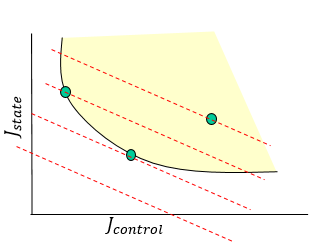
\includegraphics[width=0.5\textwidth]{cost-tradeoff.PNG}\\
  \caption{Tradeoff in the cost of state and control}\label{fig:L12-cost-tradeoff}
  \end{centering}
\end{figure}


\paragraph{Movement cost problem}\ \\

Assume we have the following simpler problem. We do not have any
state cost, but we only need to reach a desired final state. The
only cost is over the control $J_{control}=\sum_t \|u_t\|^2$. How
would the solution look like?

To be more concrete, consider the simple dynamics $x_{t+1}=x_t+u_t$,
which implies $A=B=I$. We are given a desired final state
$X_{final}=x_T$ and we like to set the controls.

A naive solution is to set $u_1=x_{final}-x_0$ and $u_t=0$ for
$t\geq 2$. The cost is $\|u_1\|^2=\|x_{final}-x_0\|^2$. The good
news is that it is finite, the bad news is that we can do much
better. Rather than doing the move in a single step, we can do it in
$T$ steps. We set $u_t= \frac{x_{final}-x_0}{T}$, and the cost is
$\sum_t \|u_t\|^2=T\|\frac{x_{final}-x_0}{T}\|^2=
\frac{\|x_{final}-x_0\|^2}{T}$. We gained a factor of $T$.

It is not hard to see that this is the optimal solution. First, any
solution which deviate from the line $x_{final}-x_0$ can be only
improved by projecting the controls to that line. Second, given that
we only make steps on the line, equal size steps will minimize our
costs. Namely, $u_t = \alpha_t (x_{final}-x_0)$ such that
$\alpha_t\geq 0$ and $\sum_t\alpha_t=1$, then the cost is $\sum_t
\alpha_t^2$. This is minimized at $\alpha_t=1/T$.

\subsection{Optimal LQR control}

We will use a dynamic programming approach. For each state $x_t$ we
define the cost-to-go as,
\[
J(u_t, \ldots, u_{T-1},x_t)=\sum_{i=t}^{T-1}x_i^\top Qx_i+u_i^\top R
u_i+ x_T^\top Q_f x_T
\]
Any optimal solution for times $[1,T]$ is also an optimal solution
for any suffix $[t,T]$.

We define the optimal value function $V^*_t(x_t)$ from state $x_t$
at time $t$ until time $T$. Our optimization problem is
\[
V^*_0(x_0)=\min_{u_0, \ldots, u_{T-1}} J(u_0, \ldots, u_{T-1},x_0)
\]
At any time $t$ we have
\[
V^*_t(x_t)=x_t^\top Qx_t +(u_t^*)^\top R u_t^*
+V^*_{t+1}(Ax_t+Bu_t^*)
\]
where
\[
u_t^*= \arg\min_u x_t^\top Qx_t +u^\top R u +V^*_{t+1}(Ax_t+Bu)
\]
We construct the optimal control sequence and value functions by
backward derivation from time $t=T$ to time $t=0$.

The main theorem will show how to compute the optimal controls.
\begin{theorem}
The optimal cost-to-go and optimal control at time $t$ is,
\[
V^*_t(x_t)=x_t^\top P_t x_t \;\;\;\; u_t^*=-K_t x_t
\]
where $P_T=Q_f$ and
\[
P_t=Q+K_t^\top RK_t +(A-BK_t)^\top P_{t+1} (A-BK_t)
\]
\[
K_t = (R+B^\top P_{t+1} B)^{-1}B^\top P_{t+1}A
\]
and $P_t$ is a p.s.d. symmetrix matrix.
\end{theorem}

The theorem has a few interesting implications. Optimal cost-to-go
is a quadratic function of state $x_t^\top P_t x_t$. The optimal
control is linear in state $u_t=-K_t x_t$. (See a numeric example in
the slides.)

\begin{proof}
The proof is by backward induction from $t=T$ to $t=0$. We will also
claim that $P_t$ is symmetric and positive semi-definite.

For the base of the induction, $t=T$, we have $P_T=Q_f$ and
$V^*_T(x_T)=x_T^\top Q_f x_T$. (Clearly, $P_T$ is p.s.d. since $Q_f$
is.)

For the induction step, assume the inductive hypothesis holds for
$t$ and we show it for $t-1$.

We have,
\[
V^*_{t-1}(x_{t-1})=\min_u x_{t-1}^\top Qx_{t-1} +u^\top R u
+V^*_{t}(Ax_{t-1}+Bu)
\]
By the inductive hypothesis $V^*_{t}(Ax_{t-1}+Bu)=(Ax_{t-1}+Bu)^\top
P_t(Ax_{t-1}+Bu)$, and we have
\[
V^*_{t-1}(x_{t-1})=\min_u x_{t-1}^\top Qx_{t-1} +u^\top R u
+(Ax_{t-1}+Bu)^\top P_t(Ax_{t-1}+Bu)
\]
We can now solve for $u$:
\[
\nabla_u V_{t-1}^*(x_{t-1})=2u^\top R+2(Ax_{t-1}+Bu)^\top P_t B=0
\]
which implies that
\[
u_{t-1}^*=-(R+B^\top P_tB)^{-1}B^\top P_t A x_{t-1}=-K_{t-1}x_{t-1}
\]
Since $P_t$ is a p.s.d. matrix,  then $R+B^\top P_t B$ is a p.s.d.
matrix. If $R$ is full rank then we have an inverse.
%
This completes the
part that $u_{t-1}$ is linear in $x_{t-1}$.

We now need to compute the value function.
%
\begin{align*}
V^*_{t-1}(x_{t-1}) =& x_{t-1}^\top Qx_{t-1}+(u^*_{t-1})^\top
Ru^*_{t-1} +(Ax_{t-1}+Bu^*_{t-1})^\top P_t (Ax_{t-1}+Bu^*_{t-1})\\
=&x_{t-1}^\top Qx_{t-1}+(K_{t-1}x_{t-1})^\top
RK_{t-1}x_{t-1} +(Ax_{t-1}-BK_{t-1}x_{t-1})^\top P_t (Ax_{t-1}-BK_{t-1}x_{t-1})\\
=& x_{t-1}^\top \left(Q+K^\top_{t-1}RK_{t-1}+(A-BK_{t-1})^\top P_t
(A-BK_{t-1})\right)x_{t-1}\\
=& x_{t-1}^\top P_{t-1}x_{t-1}
\end{align*}
where $P_{t-1}=Q+K^\top_{t-1}RK_{t-1}+(A-BK_{t-1})^\top P_t
(A-BK_{t-1})$. Since $P_{t-1}$ is the sum of p.s.d. matrices, it is
p.s.d matrix. Since $P_t$ is symmetric, $P_{t-1}$ is also symmetric,
i.e., $P_{t-1}=P^\top_{t-1}$.
\end{proof}


\section{LQR: Discrete time infinite horizon}

Assume that the horizon is $T=\infty$. The value function is,
\[
V_0^*(x_0)=\min_{u_0,\ldots} \sum_{t=0}^\infty x_t^\top Q x_t
+u_t^\top R u_t
\]
where $x_{t+1}=Ax_t+Bu_t$.

First, since we have an infinite sum, we need to ask whether the
costs are finite. In the case that we can reach $x_t=0$, then
afterwards, we have that the costs are zero, so the sum is finite.

Similar to the finite horizon case, we have,
\begin{theorem}
There exists matrices $P$ and $K$ such that the optimal cost-to-go
and optimal control at time $t$ is,
\[
V^*_t(x_t)=x_t^\top P x_t \;\;\;\; u_t^*=-K x_t
\]
\end{theorem}

The Bellman's optimality equation states,
\begin{align*}
V^*(x)=& \min_u  x^\top Qx + u^\top Ru+V^*(Ax+Bu)\\
=& \min_u  x^\top Qx + u^\top Ru+(Ax+Bu)^\top P(A+Bu)
\end{align*}
Minimizing over $u$ we have
\begin{align*}
\nabla_u V^*(x)=&  2 u^\top R+2(Ax+Bu)^\top P=0\\
u^*=& -(R+B^\top PB)^{-1}B^\top PAx=-Kx
\end{align*}

The optimal value function is
\begin{align*}
V^*(x)=& x^\top Px\\
=& x^\top Qx + (u^*)^\top Ru^*+(Ax+Bu^*)^\top P(A+Bu^*)\\
=& x^\top (Q+A^\top P A - A^\top P B(R+B^\top P B)^{-1} B^\top P A)x
\end{align*}

Since this holds for any $x$ we have
\[
P=Q+A^\top P A - A^\top P B(R+B^\top P B)^{-1} B^\top P A
\]
which is called the Algebraic Riccati Equation (ERA).


\section{Controllability}

Controllability, is define as the ability to reach from any initial
state $x_0$ any final state $x_D$, after a large enough time $T$. If
the system is controllable, then there exist a solution to the ARE.

Consider how the system evolves:
\begin{align*}
x_{t+1}=& Ax_t+Bu_t\\
=& A(Ax_{t-1}+Bu_{t-1})+Bu_t\\
=&A^2x_{t-1}+ABu_{t-1}+B_{u_t}\\
=& A^3 x_{t-2}+A^2B u_{t-2}+AB u_{t-1}+Bu_t\\
=&A^{t+1} x_0+\sum_{i=0}^{t} A^i B u _{t-i}
\end{align*}

We can define now a matrix $C$ and vector $U$, where
\[
C=[ B\; AB\; A^2B \cdots A^t B] \;\;\; U=[u_t^\top \;u_{t-1}^\top
\cdots u_0^\top]
\]
and we have
\[
x_{t+1}=A^{t+1}x_0 +CU
\]
Therefore a sufficient condition for controllability is to have $C$
full rank. This will ensure that we can enforce that $x_{t+1}=x_D$
for any $x_D$ (by solving the linear equations).

The next question is how large a $t$  we need? Recall that the
states are $x\in \mathbb{R}^n$. We will claim that $t=n-1$ will be
sufficient.

The Cayley-Hamilton theorem states that for any matrix $A$, we have
that $A^n$ is linearly dependent on $A^i$ for $i<n$. One proof is to
consider the characteristic polynomial $p(\lambda)=det(\lambda I
-A)=\sum_{i=0}^n c_i \lambda^i$, where $c_n=1$. Since setting
$\lambda=A$ we get the zero matrix, which implies that
$A^n=\sum_{i=0}^{n-1}-c_i A^i$.) This implies that a sufficient
condition is that the following matrix is full rank
\[
C=[ B\; AB\; A^2B\; \cdots A^{n-1} B]
\]
This also guarantees that the ARE has a solution. (See the slides
for examples)

\section{LQR: Stability}

Let $P$ be the solution to the ARE. Then $K=(R+B^\top P
B)^{-1}B^\top PA$ and $u^*=-Kx$.

Consider the dynamics of the optimal control.
\begin{align*}
x_{t+1} =& Ax_t + Bu_t\\
=& Ax_t -BKx_t\\
=& (A-BK)x_t\\
=&(A-BK)^{t+1}x_0
\end{align*}

Consider the eigenvalues of the matrix $A-BK$. We can write it as
\[
A-BK=M\Lambda M^{-1}
\]
where $\Lambda$ is a diagonal matrix with the eigenvalues
$\lambda_i$ on the diagonal.

If for every $i$ we have $|\lambda_i|<1$ then the system converges
to zero. In such a case the system is {\em stable} and has a finite
cost.

If there exists an $i$ such that $|\lambda_i|>1$ the system diverges
and is not stable. Also, the system has infinite cost (for any
control).

\section{Extensions to LQR}

We will discuss a few extensions of the basic LQR system.
\begin{enumerate}
\item
Affine system: add a constant vector to the dynamics.
\item
Smoothness: Penalize the change in control, i.e., $u_t-u_{t-1}$.
\item
Noise: allow for Gaussian noise. Called Linear Quadratic Gaussian.
\item
Linear Time Varying (LTV) system, having matrices $A_t$ and
$B_t$.
\item
Non-Linear system: Linearize the system
\end{enumerate}

\subsection{LQR: Affine system}

We define a new dynamics, where there is an additional constant
vector $c\in\mathbb{R}^n$. Namely,
\[
x_{t+1}=Ax_t+Bu_t+c
\]
The cost is as before $x_t^\top Qx_t+u_t^\top Ru_t$.  We an affine
system the control remains linear. One way to show that is to redo
all the math. A simpler option is a reduction.
\[
\begin{bmatrix}
x_{t+1}\\
1
\end{bmatrix}
=\begin{bmatrix}
A&c\\
0&1
\end{bmatrix}
\begin{bmatrix}
x_{t}\\
1
\end{bmatrix}+
\begin{bmatrix}
B\\
0
\end{bmatrix}
u_t
\]
This implies that we have a new state $z_t=\begin{bmatrix}
x_{t}\\
1
\end{bmatrix}$, and the new dynamics become
\[
z_{t+1}=A'z_t+B'u_t
\]
We can now apply everything we know about the LQR. We get that the
optimal control $u^*_t$ is linear in $z_t$ and hence linear in
$x_t$.

\subsection{LQR: Smoothness}

We would like to penalize for changing the control. Let $\Delta
u_t=u_t-u_{t-1}$. Our new cost becomes
\[
x^\top_t Qx_t +u_t^\top R u_t + (\Delta u_t)^\top R' \Delta u_t
\]
and the dynamics remain $x_{t+1}=A x_t + B u_t$.

We can reduce this case also to the standard LQR.
\[
\begin{bmatrix}
x_{t+1}\\
u_t
\end{bmatrix}
=\begin{bmatrix}
A&B\\
0&1
\end{bmatrix}
\begin{bmatrix}
x_{t}\\
u_{t-1}
\end{bmatrix}+
\begin{bmatrix}
B\\
I
\end{bmatrix}
\Delta u_t
\]
This implies that we have a new state $z_t=\begin{bmatrix}
x_{t}\\
u_{t-1}
\end{bmatrix}$, and the new dynamics become
\[
z_{t+1}=A'z_t+B'u_t
\]
and cost $Q'$ and $R'$ where
\[
Q'=\begin{bmatrix}Q & 0\\ 0 & R\end{bmatrix}
\]
and the cost is
\[
\sum_{t=0}^\infty z_t^\top Q'z_t+(\Delta u_t)^\top R' \Delta u_t =
\sum_{t=0}^\infty x_t^\top Qx_t+u_{t-1}^\top R u_{t-1}+(\Delta
u_t)^\top R' \Delta u_t
\]


\subsection{Linear Quadratic Gaussian (LQG)}

We add a Gaussian noise to the dynamics,
\[
x_{t+1}=A x_t + B u_t +w_t
\]
where $w_t \sim N(0,W)$ for a correlation matrix $W\in
\mathbb{R}^{n\times n }$.

We have the same objective, but now we like to minimize the expected
cost. Note that now the expected cost in each time is none zero (due
to the noise).

For a finite horizon we have
\[
V^*_t(x_t)= x_t^\top P_t x_t + m_t
\]

 We will show this by
backward induction on $t$. For $t=T$ we have $V_T^*(x)=x^\top Q_fx$.
Assume it holds for $t$ and we show it for $t-1$.
\[
V^*_{t-1}(x_{t-1})=\min_{u_{t-1}} x_{t-1}^\top Qx_{t-1}+u_{t-1}^\top
Ru_{t-1}+E_{w_t\sim N(0,W)}[V^*_t(Ax_{t-1}+Bu_{t-1}+w_t)]
\]
By the induction hypothesis, we have
\[
E[V^*_t(x_t)]=E[(Ax_{t-1}+Bu_{t-1}+w_t)^\top P_t
(Ax_{t-1}+Bu_{t-1}+w_t)]+m_t
\]
This implies that
\[
V^*_{t-1}(x_{t-1})=\min_{u_{t-1}} x_{t-1}^\top Qx_{t-1}+u_{t-1}^\top
Ru_{t-1}+(Ax_{t-1}+Bu_{t-1})^\top P_t (Ax_{t-1}+Bu_{t-1})+m_{t-1}
\]
where $m_{t-1}=m_t +Tr(WP_t)=m_t +\sum_{i,j} W[i,j]P_t[i,j]$.

Note that the solution to the LQG is identical to that of the LQR.

Solving for the optimal control we have
\begin{align*}
\nabla_{u_{t-1}} V^*_{t-1}(x_{t-1}) =&
2u_{t-1}R+2(Ax_{t-1}+Bu_{t-1})^\top P_t B =0\\
u_{t-1}^*=& -(R+B^\top P_t B)^{-1}B^\top P_t Ax_{t-1}\\
V^*_{t-1}(x_{t-1})=&x_{t-1}^\top P_t x_{t-1} + m_{t-1}
\end{align*}
where $m_{t-1}=Tr(WP_t)+m_t$ and $m_T=0$.

\subsection{Time Varying System}

We assume that $x_{t+1}=A_t x_t +B u_t$. The cost is still $x_t^\top
Qx_t+u_t^\top Ru_t$.

The math is very similar to before and we get
\[
u_t^*=-K_t x_t
\]
and
\[
V^*_t(x_t)=x_t^\top P_t x_t
\]

\subsection{Non-linear system}

Assume a general non-linear dynamics
\[
x_{t+1}=f(x_t,u_t)
\]

Assume that the goal is to stabilize the system at state $x^*$.
Clearly we need a control $u^*$ such that $x^*=f(x^*,u^*)$.

The first step would be linearizing the system around $x^*$. Using
Taylor expansion we have
\[
x_{t+1}\approx f(x^*,u^*)+A(x_t-x^*)+B(u_t-u^*)
\]
where the matrices $A$ and $B$ are the partial derivatives of
$f(x^*,u^*)$ with respect to $x$ and $u$.

We can now reduce the approximate system to LQR. Let the state be
$z_t=x_t-x^*$. Let the control be $v_t=u_t-u^*$. We have that
$z_{t+1}=Az_t + Bu_t$ and the cost is $z_t^\top Qz_t+v_t^\top Rv_t$.
This implies that the optimal control is $v_t = -Kz_t$. By
substituting the values we have $u_{t+1}-u^*=-K(x_{t}-x^*)$, which
becomes,
\[
u_{t+1}=u^*-K(x_t-x^*)
\]

When is such a linearization likely to be successful. We need a good
approximation for both $x^*$ and $u^*$.

\section{System Estimation}

So far we have looked only at planning, given a model find the
optimal policy. What happens when the model is unknown?

We will consider a simple  model based approach. We estimate the
system parameters $A$ and $B$. Given the estimated $A$ and $B$ we
can compute the optimal policy.

We will look at two methods, both involving least squares. The first
is an offline method, using ordinary least squares. The second is an
online method, which is called also recursive least squares.



\subsection{Ordinary Least Squares}

Assume we observe a system trajectory $(x_t,u_t)_{t=0}^T$. The
system dynamics are $x_{t+1}=Ax_t+B u_t$, where the unknowns are $A$
and $B$.

We can solve for the $A$ and $B$ using a least squares method
\[
\min_{A,B} \sum_t \| x_{t+1}-(Ax_t+Bu_t)  \|^2
\]
We can treat this as a regression problem. Define
$M=\begin{bmatrix}A\\ B\end{bmatrix}$ and $z_t =[x_t\; u_t]$ (note
that $z_t$ is a row vector). Set,
\[
Z=\begin{bmatrix}z_0\\ \vdots\\z_{T-1}\end{bmatrix}\;\;\; X=
\begin{bmatrix}x_1\\ \vdots\\x_{T}\end{bmatrix}
\]
We have that $X\approx Z M$. The least square solution is
$\hat{M}=(Z^\top Z)^{-1}Z^\top X$, assuming $Z^\top Z$ is
invertible.

\subsection{Recursive Least Squares}

The idea is to keep continuously updating the matrix $\hat{M}$ as we
get more observations. Let
\[
\hat{M}_t = (Z_t^\top Z_t)^{-1}Z_t^\top X_t=\Phi_t^{-1}\Psi_t
\]
where $\Phi_t=Z_t^\top Z_t=\sum_{i=1}^t z_i^\top z_i$ and
$\Psi_t=Z_t^\top X_t=\sum_{i=1}^t z_i^\top x_i$.

We can now update the parameters as follows:
\begin{align*}
\Phi_{t+1}^{-1}=&(\Phi_t+z_t^\top z_t)^{-1} =
\phi_t^{-1}-\frac{\Phi_t^{-1}z_{t+1}z_{t+1}^\top\Phi_t^{-1}}{1+z_{t+1}^\top\Phi_t^{-1}z_{t+1}}\\
\Psi_{t+1}=&\Psi+z_{t+1}^\top x_{t+1}\\
\hat{M}_{t+1}=&\Phi_{t+1}^{-1}\Psi_{t+1}
\end{align*}



\section{Bibliography Remarks}

The lecture borrows from the scribe note of
\href{https://courses.cs.washington.edu/courses/cse599i/18wi/resources/lecture20/lecture20.pdf}{Kevin
Jamieson}.


The autonomous helicopter is from Abbeel et al. \cite{AbbeelCN2010}

%\bibliography{../bib-lecture}
%\bibliographystyle{plain}
